\chapter{Teoretická část}\label{chap:teorie}

Tato kapitola je věnována přiblížení teoretického kontextu této práce.

\section{Virtualizace}\label{sec:virtualization}

Koncept virtualizace se poprvé objevil na konci 50.\,let minulého století, kdy skupina z University v Manchesteru vytvořila první funkční prototyp virtuální paměti. Následně v 60.\, letech minulého století byl koncept rozšířen i na celé počítače. První tzv. \textit{virtual machine} (VM), neboli česky \uv{virtuální stroj}, byl vytvořen firmou IBM a jeho cílem bylo umožnit souběžný přístup k sálovým počítačům. Každá VM byla instancí fyzického stroje a dávala iluzi toho, že uživatel přistupuje přímo k fyzickému stroji. Uživatelé mohli vyvíjet, spouštět a testovat aplikace bez obav z toho, že by se mohl zhroutit celý počítač, díky tomu, že každá VM byla izolovanou kopií systému. 

V polovině 70.\,let minulého století byla virtualizace již dobře akceptovaným konceptem mezi uživateli. Použitím virtualizace totiž mohli vyřešit podstatné problémy této doby. Například díky již zmíněné virtualizované paměti mohli uživatelé adresovat mnohem větší operační paměť, než počítač skutečně obsahoval. 

Všechny tyto virtualizační techniky byly primárně cestou k vyrovnání se s vysokou pořizovací cenou hardwaru v této době. Díky tomu mohli majitelé sálových počítačů využít svoji investici co nejefektivněji. Jejich použití se tedy se snižujícími cenami hardwaru začalo snižovat a dokonce skoro vymizelo během 80. a 90.\,let díky příchodu levnějších osobních počítačů.  

Poptávka po virtualizaci začala znovu růst až v 90.\,letech minulého století. Se zvětšující se různorodostí hardwaru a softwaru zde vznikla poptávka na schopnost spustit aplikace, které byly původně určeny pro jiný hardware a jiný operační systém, na jednom určitém stroji. 

Poptávka se ovšem zvětšila i v komerčním sektoru. S zvyšujícími se počty serverů firmy hledaly způsoby, jak využít tuto investici do serveru naplno. Spustit pouze jednu aplikaci na serveru nebylo příliš ekonomické, jelikož tato aplikace nemusela vždy využít všechny výpočetní zdroje, a nákup dalších serverů přinášel mimo samotné pořizovací ceny i další náklady, například na údržbu a administraci. Řešením tohoto problému byla opět virtualizace. Oba tyto trendy pokračují dodnes a patří mezi hlavní důvody pro dnešní využití virtualizace. 

Virtualita se od reality liší pouze ve formálním světě. Má ovšem podobné jádro nebo efekt. V počítačovém světě je virtualizované prostředí vnímáno aplikací stejně jako reálné prostředí, přestože některé mechanismy v něm mohou fungovat jinak. Toto prostředí hlavně dává aplikaci zkreslený obraz reálného stroje, přičemž v tomto zkresleném obraze může mít stroj více či méně určitých zdrojů. Typický moderní počítač využívá spoustu takovýchto přístupů. Jedním příkladem je již zmíněná virtuální paměť, díky níž může proces použít mnohem více paměti, než je fyzicky dostupné. Tato virtuální paměť taktéž umožňuje sdílení fyzické paměti mezi stovkami procesů. Podobným konceptem je i multitasking, kdy jeden procesor je rozdělen a prezentován jako \uv{virtuální procesor} jednotlivým procesům. Na druhou stranu, několik procesorů může být seskupeno do jednoho výkonnějšího virtuálního procesoru.

Možností virtualizace je tedy spousta, a to na mnoha úrovních. Virtualizaci tedy můžeme nadefinovat takto:

\begin{displayquote}
    Virtualizace je technologie, která kombinuje/rozděluje, výpočetní zdroje k prezentaci jednoho či více prostředí za pomoci metodologií jako hardwarového a softwarového rozdělování/agregování, parciální/kompletní simulací stroje, emulace a spousty dalších.
\end{displayquote}

Jak je z definice vidět, virtualizace není jen o rozdělování výpočetních zdrojů, ale i o jejich sjednocování do větších celků. V rámci této práce se ale zaměřuji primárně na rozdělování výpočetních zdrojů za pomoci virtualizace. Mezi praktické využití virtualizace může patřit například:

\begin{description}
    \item[Konsolidace serveru] Za pomoci virtualizace lze přerozdělit práci z více serverů, které nejsou na plno používány, na jeden server, a tím ušetřit na hardwaru, managementu a administraci infrastruktury. Díky ní tedy snižujeme komplexitu administrace, jelikož veškerý software ve VM je nezávislý na softwaru fyzického serveru. 
    \item[Sandbox] Za pomoci virtualizace lze vytvořit bezpečné a hlavně izolované prostředí pro běh aplikací, jejichž původ nám může být neznámý a spuštění v normálním prostředí počítače by mohlo představovat bezpečnostní riziko. Tato technika se označuje jako \textit{sandboxing}.
    \item[Virtuální hardware] Virtualizace může zprostředkovat hardware, který počítač nikdy neměl. Mezi ně patří například virtuální ethernetové adaptéry, switche, huby atd.
    \item[Spuštění více OS] Bez virtualizace nejsme schopni spustit více operačních systémů zároveň. Virtualizace tedy přináší prostředky, jak toto umožnit. Mimo to ale také přináší prostředky, jak spustit staré operační systémy na novém hardwaru, pro který daný operační systém nemusel být vyvinut.
    \item[Testování/QA] S pomocí virtualizace jsme schopni vytvořit libovolné testovací scénáře, které jinak mohou být těžce simulovatelné v reálném světě. 
\end{description}

Jak je vidět z tohoto krátkého seznamu, důvodů proč virtualizovat je spousta. Jak ale virtualizace funguje? V praxi je virtualizace abstrakční vrstva, která poskytuje potřebné propojení mezi dvěma izolovanými vrstvami. Toto si lze lépe představit pomocí obrázku \ref{fig:pc_stack}, na kterém lze spatřit zjednodušenou architekturu počítače. Je zde vidět, že virtualizační vrstvu lze vložit mezi jakékoliv dvě vrstvy a tím docílit virtualizace. \cite{campbell2006introduction}\cite{chiueh2005survey}

\begin{figure}[htbp]
    \centering 
    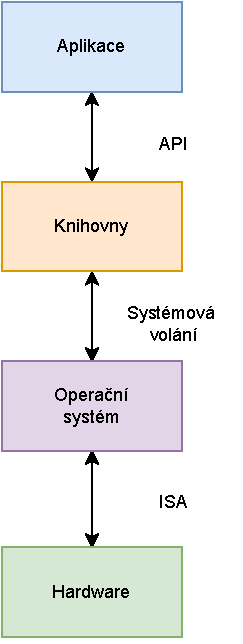
\includegraphics[width=0.325\textwidth]{assets/img/computer_stack.pdf}
    \caption{Architektura počítače ukazující příležitosti k virtualizaci}
    \source{Vytvořeno dle předlohy z \cite{chiueh2005survey}}
    \label{fig:pc_stack}
\end{figure}

V případě dnes nejpopulárnější architektury x86 je potřeba i rozlišit, s jakými právy daná virtualizace běží. Architektura x86 definuje tzv. \textit{protekční kruhy}, kde každý kruh(anglicky se tyto úrovně označují jako \textit{ring}), neboli úroveň, definuje, co daná aplikace může a nemůže udělat. Grafickou představu těchto úrovní můžeme vidět na obrázku \ref{fig:priv_rings}. Jak je vidět, čím nižší úroveň, tím více práv software běžící v této úrovni má. Typicky v úrovni 0 běží operační systém, v úrovních 1 a 2 systémové ovladače, a v úrovni 3 tři samotné aplikace. \cite{RODRIGUEZHARO2012267}

\begin{figure}[htbp]
    \centering 
    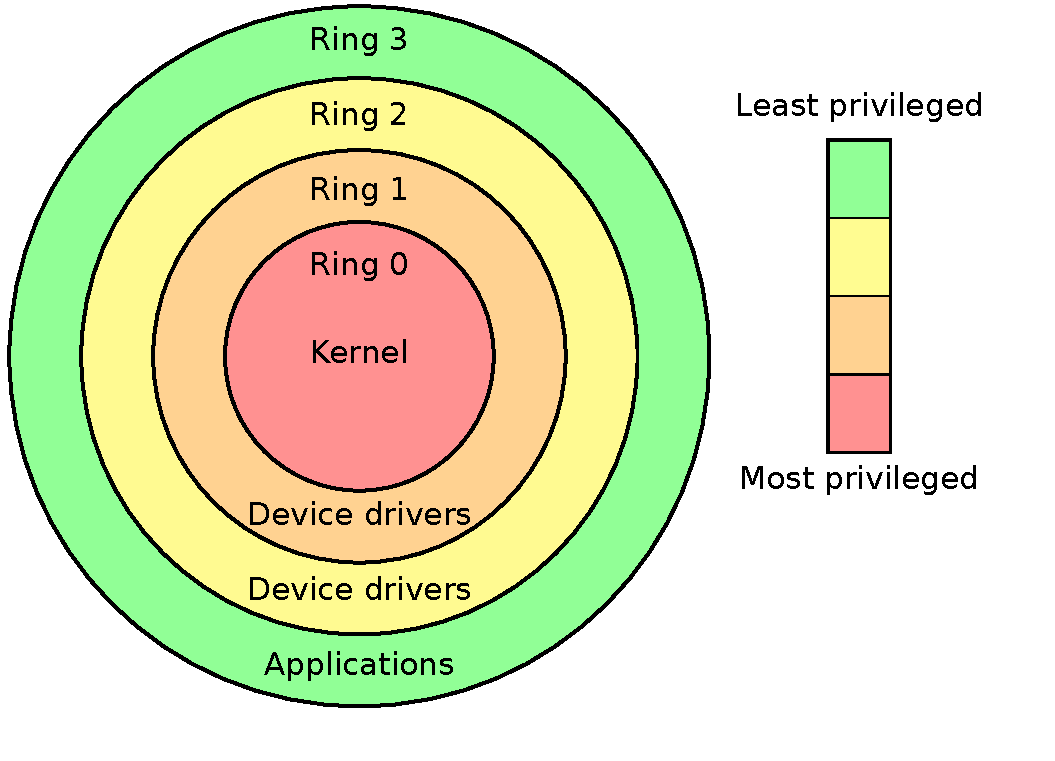
\includegraphics[width=\textwidth]{assets/img/priv_rings.pdf}
    \caption{Architektura počítače ukazující příležitosti k virtualizaci}
    \source{Wikipedia Commons \cite{privrings}}
    \label{fig:priv_rings}
\end{figure}

\subsection{Hypervizor}

Důležitou komponentou při virtualizaci je tzv. \textit{hypervizor} (někdy také označován jako Virtual Machine Monitor - VMM). Hypervizor je softwarová vrstva, která virtualizuje všechny potřebné zdroje fyzického stroje, a tím definuje a podporuje běh jednoho či více VM. \cite{whitaker2002denali}

Existují dva typy hypervizorů. Ty můžeme vidět na obrázku \ref{fig:vm_types}. Hypervizor typu I běží přímo nad hardwarem a spravuje všechny virtuální stroje. Díky tomu hypervizor může mít plnou kontrolu nad hardwarem, jelikož běží v úrovni nejvyšší priority. Hypervizor typu 2 běží nad hostitelským operačním systém, respektive uvnitř něj. Tento hypervizor je odkázán na hostitelský systém, který mu přiděluje prostředky, jelikož každá VM je v podstatě další proces v systému.\cite{chiueh2005survey}\cite{RODRIGUEZHARO2012267}

\begin{figure}[htbp]
    \centering 
    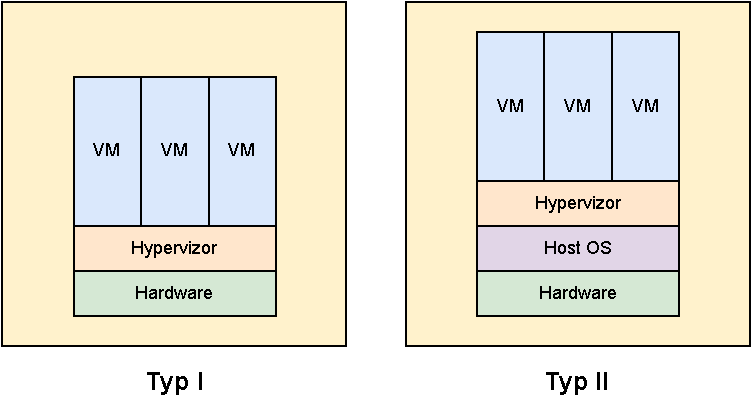
\includegraphics[width=\textwidth]{assets/img/vm_types.pdf}
    \caption{Možné typy virtualizace na úrovni HAL}
    \source{Vytvořeno dle předlohy z \cite{RODRIGUEZHARO2012267}}
    \label{fig:vm_types}
\end{figure}

\subsection{Možnosti virtualizace z technologického pohledu}

Jak již bylo nastíněno, virtualizační vrstva může existovat na více úrovních. V této sekci bude přiblížena virtualizace od nejnižší vrstvy až po tu nejvyšší.

\subsubsection{Virtualizace ISA}

ISA, neboli \textit{Instruction Set Architecture} je součástí abstraktního modelu počítače a definuje, jak může software ovládat procesor. ISA funguje jako rozhraní mezi hardwarem a softwarem a specifikuje, co a jak je procesor schopen udělat.\,\cite{isa-arm}

Virtualizace na této úrovni tedy funguje za pomoci softwarové emulace ISA dané platformy. Tedy virtuální vrstva musí být schopna přeložit ISA instrukce hosta na ISA instrukce hostitele. Tento způsob lze označit i jako \textit{binární překlad}. Tato virtualizace funguje pouze v případě, že existuje způsob, jak na hostitelské platformě provést všechny úkony požadované architekturou hosta. 

Výhodou této virtualizace je, že nám teoreticky dokáže dát dostatečné prostředky ke spuštění jedné platformy (jako například x86) na ostatních platformách. Taktéž jsme schopni spustit operační systémy bez jakékoli modifikace. Tato portabilita ovšem přichází s nemalou cenou. Tím, že musíme každou instrukci softwarově přeložit, následně dochází k velkému snížení výkonu systému. I tak si tento způsob virtualizace však nalezne využití. \cite{chiueh2005survey}\cite{RODRIGUEZHARO2012267}


\subsubsection{Virtualizace HAL}

Hardware abstraction layer (HAL), neboli česky hardwarová abstrakční vrstva, je vrstva, která vytváří jednotné API pro přístup k hardwaru. Díky ní je možné oddělit implementaci přístupu k hardwaru od samotného softwaru. Software totiž pouze využívá API definované HAL a až následná implementace na daném zařízení definuje reálný přístup k hardwaru daného stroje. \cite{haldef}

Virtualizace HAL tedy využívá podobnosti mezi architekturou platformy hosta a hostitele, díky čemuž je snížena latence způsobená překladem. Často je ovšem spojována společně s binárním překladem. Ten může nastat například z důvodu nedostatečných práv k vykonání operace v rámci úrovně, ve které hypervizor běží. \cite{chiueh2005survey}\cite{vcc_2}


\subsubsection{Virtualizace na úrovni programovacího jazyka}

Virtualizace na úrovni programovacího jazyka probíhá v rámci aplikační vrstvy. Ideou bylo vytvořit virtuální stroj již na aplikační úrovni, který oddělí aplikaci od hardwaru. Implementace tohoto aplikačního virtuálního stroje následně definuje reálný přístup k výpočetním zdrojů. K těm je přistupováno standardizovaným způsobem, jenž je definován abstrakční vrstvou. Pro představu lze uvést například Java Virtual Machine, nebo Common Language Runtime v .NET Frameworku. \cite{chiueh2005survey}


\subsubsection{Virtualizace na úrovni knihoven}

Virtualizace na úrovni knihoven může připomínat předchozí popsanou virtualizaci, ovšem důležitá je změna původu této implementace. Každá aplikace využívá volání různých externích zdrojů. Tyto zdroje mohou a nemusí být přenositelné mezi operačními systémy. Virtualizace na této úrovni využívá rozhraní daných externích zdrojů, ovšem implementace je přizpůsobena tomu stroji, na kterém aplikace běží. Jako příklad lze uvést například Wine, který implementuje Windows API v UNIX prostředí. 


\subsection{Virtualizační techniky}

V následující sekci jsou přiblíženy reálné přístupy k virtualizaci, které používají buď jednu z předem zmíněných virtualizačních technik, nebo tyto techniky kombinují. 

\subsubsection{Plná virtualizace}

Plná virtualizace funguje na principu kombinace přímého spuštění instrukcí a binárního překladu instrukcí za běhu. Využívá se toho, že hypervizor běží na nulté úrovni, tedy s nejvyšší prioritou a s největšími právy. Hypervizor tím pádem zcela odděluje operační systém od skutečného hardwaru. Toto lze vidět na obrázku \ref{fig:full_virt}.\cite{4709159}

\begin{figure}[htbp]
    \centering 
    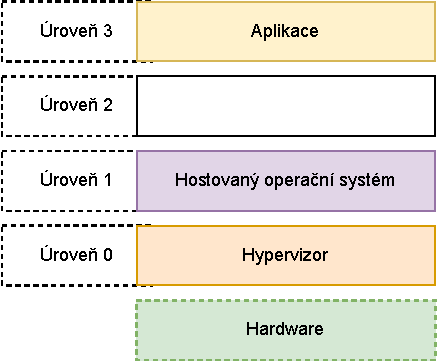
\includegraphics[width=0.65\textwidth]{assets/img/full_virt.pdf}
    \caption{Plná virtualizace}
    \source{Podle \cite{vcc_2}}
    \label{fig:full_virt}
\end{figure}


\subsubsection{Paravirtualizace}

Paravirtualizace funguje na stejných úrovních jako plná virtualizace. Hypervizor má plnou kontrolu nad hardwarem hostitelského stroje a operace s ním jsou zprostředkovávány hypervizorem. Změna ovšem nastává v rámci operačního systému. Ten má totiž upravené jádro a díky tomu ví, že běží v paravirtualizovaném prostředí. Jednotlivá ISA volání jsou tedy nahrazena voláním virtualizačních funkcích. Tedy operační systém přímo komunikuje s hypervizorem.\cite{4709159}


\subsubsection{Hardwarově asistovaná virtualizace}

Hardwarově asistovaná virtualizace funguje na principu přímé podpory virtualizace ze strany hardwaru. V rámci této virtualizace je mezi protekční vrstvy přidána nová vrstva na úroveň -1, tedy pod všechny ostatní úrovně. Privilegované instrukce jsou tedy zachyceny přímo hardwarem a následně jsou předány hypervizoru ke zpracování.\cite{4709159}

\begin{figure}[htbp]
    \centering 
    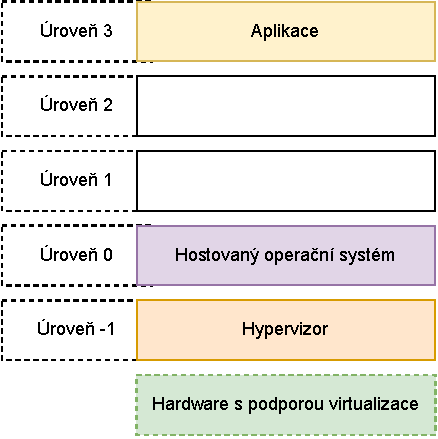
\includegraphics[width=0.65\textwidth]{assets/img/hardware-asssist-virt.pdf}
    \caption{Hardwarově asistovaná virtualizace}
    \source{Podle \cite{vcc_2}}
    \label{fig:hardware_asssist_virt}
\end{figure}

\subsubsection{Kontejnerová virtualizace}

Kontejnerová virtualizace, neboli zkráceně kontejnerizace, je lehčí alternativou k tradiční virtualizaci. Porovnání s tradiční virtualizací můžeme vidět na obrázku \ref{fig:containerization}. Tradiční VM jsou nahrazeny tzv. \textit{kontejnery}. Jak je vidět, kontejnery již nemusí obsahovat kopii celého operačního systému. Kontejnery totiž sdílí jádro operačního systému a další zdroje, jako například knihovny. Díky tomu mohou být spouštěny mnohem rychleji než VM. \cite{8693491}

Všechny kontejnery jsou následně orchestrovány tzv. \textit{kontejnerizátorem}, v angličtině \textit{container engine}. Ten má na starost vše spojené s procesem spouštění a běhu kontejneru. Díky němu je mimo jiné možné rychle a efektivně propojit kontejnery mezi sebou.\cite{Bentaleb2021} 

To, co kontejnery činí tak efektními, je však zároveň i jejich nevýhodou. Sdílením jádra může docházet k bezpečnostním rizikům, kvůli čemuž jsou méně bezpečné než tradiční VM.\cite{6498558}

Nástroje, které umožňují kontejnerovou virtualizaci můžeme dle Aleksic\cite{docker_alt_23} rozdělit do čtyř kategorií:

\begin{description}
    \item[Image builders] Nástroje, které umožňují vytvářet kontejnery v souladu s pravidly dle OCI.
    \item[Container managers] V širším smyslu tak můžeme nazvat všechny nástroje, které pomáhají se sestavováním a během kontejnerů. Specificky ale tak můžeme nazvat ty nástroje, které pomáhají spravovat jednotlivé instance kontejnerů.
    \item[Container runtimes] Nástroje, které se starají o běh kontejnerů.
    \item[Container engines] Nástroje, které se starají o všechny procesy spojené s  kontejnerizací.
\end{description}

K úspěšnému využití kontejnerizace je samozřejmě potřeba spravovat veškeré procesy spojené s kontejnerizací. 

\begin{figure}[htbp]
    \centering 
    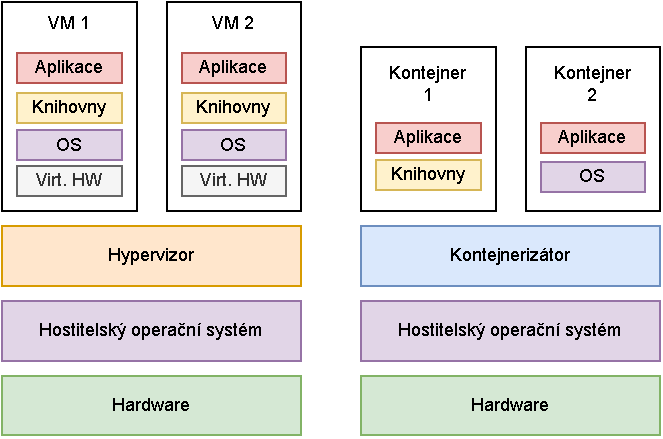
\includegraphics[width=0.9\textwidth]{assets/img/containerization.pdf}
    \caption{Porovnání virtualizace s hypervizorem oproti virtualizaci kontejnerizací}
    \source{Podle \cite{vcc_2}}
    \label{fig:containerization}
\end{figure}


\subsection{Virtualizační řešení}

V předchozích sekcích byly představeny možnosti, jak lze virtualizovat. Následující sekce jsou věnované vybraným řešením, které dnes pro virtualizaci existují.

\subsubsection{QEMU}
QEMU je emulátor, který využívá dynamického binárního překladu. Tento nástroj podporuje dva operační módy:

\begin{enumerate}
    \item Emulace uživatelského prostoru
    \item Emulace celého systému
\end{enumerate}

Za pomoci prvního módu je QEMU schopno spustit aplikaci, která byla zkompilována pro jeden procesor na jiném procesoru. V druhém emuluje celý hostovaný systém. QEMU podporuje velikou řadu procesorových architektur, jako například x86 nebo ARM. 

QEMU funguje tak, že za běhu překládá instrukce do tvaru, který vyžaduje hostující systém. Hlavní ideou je, že každá instrukce je rozdělená na několik jednodušších instrukcí, které se nazývají \textit{micro operations}, neboli česky mikro operace. Každá tato zjednodušená instrukce je implementována kusem kódu napsaném v jazyce C a následně zkompilována. 

Výstupní objektový soubor je následně použit jako vstup pro vytvoření dynamického generátoru kódu. Ten je následně spuštěn a spojením několika mikro operací dokáže vygenerovat plnohodnotnou instrukci pro hostitelský stroj.\cite{chiueh2005survey}\cite{bellard2005qemu}


\subsubsection{VMware}

VMware je dnes známá technologická firma se širokou škálou produktů. To, co ale zpopularizovalo tuto firmu a její produkty, je virtualizace. Firma VMware podporuje oba dva typy hypervizorů, jež jsou k vidění na obrázku \ref{fig:vm_types}. 

Implementace hypervizoru typu I se nazývá VMware ESXi a zaměřuje se na komerční virtualizaci serveru a jím poskytnutých služeb. Dle definice typu hypervizor běží přímo nad hardwarem a tedy i přímo s ním komunikuje. Všechny VM následně běží nad tímto hypervizorem. \cite{gillis_2022}

Hypervizor typu II. poté můžeme nalézt v produktu VMware Workstation. Tento produkt je zaměřen na virtualizaci na osobním počítači. Produkt, který je nainstalován v prostoru hostujícího operačního systému, je spouštěn jako kterýkoliv jiný program. Jeho součástí ovšem je předem zmíněný hypervizor, který se stará o propojení mezi VM a hardwarem. Komunikaci s hardwarem potom hypervizor realizuje za pomoci systémových volání hostujícího operačního systému. \cite{9647226}

Oba dva tyto produkty pracují na úrovní virtualizace celého operačního systému, tedy všechny VM obsahují plnohodnotný hostovaný operační systém.

\subsubsection{Docker}
Docker je neznámějším a nejrozšířenějším nástrojem, který zprostředkovává kontejnerizaci. Proto je také ve většině případů většina ostatních nástrojů s Docker srovnávána. Docker se skládá z několika hlavních komponentů, které dohromady tvoří container engine. Mezi tyto komponenty patří

\begin{itemize}
    \item Docker Client and Server,
    \item Docker Containers,
    \item Docker Images,
    \item Docker Registries.
\end{itemize}

Docker Client and Server, jak z překladu názvu vyplývá, obsahuje klienta a server. Server dostává žádosti od klienta, které následně zpracovává. Architekturu nástroje Docker můžeme vidět na obrázku \ref{fig:docker_arch}. Důležitou komponentou je Docker Daemon, což je persistentní proces, který neustále běží na pozadí. Klient provádí komunikaci s Docker Daemon prostřednictvím definovaného REST API a ten se následovně stará o sestavování, běh a distribuci Docker kontejnerů. Docker server a klient mohou běžet na jednom stroji, ale zároveň je možné se za pomocí klienta připojit ke vzdálenému serveru. 
\cite{turnbull2014docker}\cite{docker_overview}

\begin{figure}[htbp]
    \centering 
    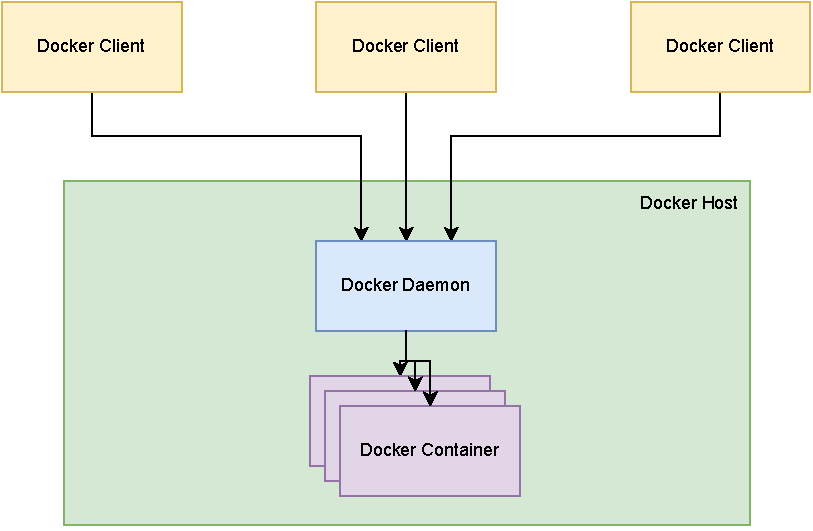
\includegraphics[width=0.97\textwidth]{assets/img/docker_arch.pdf}
    \caption{Docker architektura}
    \source{Vytvořeno dle předlohy z \cite{turnbull2014docker}}
    \label{fig:docker_arch}
\end{figure}

Jednotlivé Docker kontejnery jsou vytvářeny z tzv. Docker Images. Tyto images, neboli v češtině obrazy, obsahují definici všech závislostí a balíčků, potřebných k běhu kontejneru. Způsoby jak vytvářet obrazy jsou dva - buď můžeme definovat vlastní obraz, anebo použít nějakou již vytvořenou předlohu. Nutno podotknout, že každý existující obraz může být předlohou pro nový obraz. 

Tyto obrazy následně mohou být uloženy v Docker Registries. Ten slouží jako repozitář pro obrazy, který může být buď veřejný, nebo soukromý. Veřejný repozitář se nazývá Docker Hub\cite{docker_hub}, kde každý může získat kterýkoliv již vytvořený image, anebo může také nahrát vlastní. \cite{turnbull2014docker} 

Docker v základu nabízí několik druhů síťových ovladačů, s jejichž pomocí lze efektivně propojit kontejnery mezi sebou. Docker zároveň podporuje implementaci vlastního síťového ovladače. \cite{docker_networking_overview}

K definici prostředí Docker podporuje dva způsoby. Prvním způsobem je tzv. \textit{Dockerfile}. Dockerfile je soubor, který obsahuje všechny příkazy k vytvoření obrazu. Z takto definovaného obrazu lze následně vytvářet jednotlivé instance kontejnerů. \cite{dockerfile}

Druhým způsobem je nástroj \textit{Docker Compose}. Docker Compose umožňuje vytvořit multi-kontejnerové prostředí za pomocí definice dle formátovacího jazyku YAML. V něm lze následně definovat jednotlivé kontejnery a propojení mezi nimi. Díky tomuto přístupu je možné spouštět celé prostředí za pomoci jednoho příkazu. \cite{dockercompose}


\subsubsection{Podman}
Podman je velice podobný předchozímu řešení Docker. Tento nástroj je primárně zaměřený na operační systém Linux, kde pomáhá najít, spustit a nasadit kontejnery dle pravidel OCI. V použití je dokonce až tak podobný, že většina uživatelů může změnit příkaz \inlinecode{docker} na \inlinecode{podman} bez problémů. Rozdíly tam ale přeci jen jsou. 

Podman oproti Docker používá takzvanou \textit{daemon-less} architekturu. Jak už bylo zmíněno, Docker obsahuje neustále běžící proces, který se nazývá \textit{daemon}, jenž poslouchá příkazy od klienta a spravuje všechny procesy spojené s kontejnerizací. Tento přístup vytváří problémy hlavně z bezpečnostního hlediska, jelikož daemon musí být spuštěn s právy správce počítače. Docker sice podporuje od verze v19.03 tzv. \textit{rootless execution}, tedy mód, kdy nepotřebuje práva správce, ale při chodu v tomto módu mohou uživatelé narazit na různé limitace.

Přesně na tento problém se zaměřil Podman. Podman používá pro správu kontejnerů nástroj \textit{systemd}, který ke spuštění využívá práva uživatele, který provádí příkazy. Podman také využívá jiný nástroj \textit{Buildah}, s jehož pomocí je schopen sestavovat kontejnery bez služby daemon. 

Jak bylo řečeno na začátku, Podman je nástroj primárně zaměřený na operační systém Linux, ovšem má i svou distribuci pro Windows. Ovšem k tomu, aby mohl na Windows fungovat, musí každý kontejner obsahovat hostující systém Linux, na kterém jsou následně kontejnery spuštěny. \cite{podman}\cite{podman_vs_docker}